\subsection{Cholecystitis Pathway Variants}
This section shows the cholecystitis pathway variant plot auto-generated by ProM. Cholecystitis pathway variants are analyzed without activities from the `antibiotics' sub-process and the `monitoring labs' sub-process (see section 3.7 for the activities from the two sub-processes). Clinicians confirmed that these sub-processes are standard monitoring and maintenance systems while the patient is waiting for further diagnosis. Only analyzing activities from the primary cholecystitis pathway significantly reduces the level of clinical variation between patient traces.

The cholecystitis pathway model consists of 10 pathway variants. The 10 pathway variants from the cholecystitis pathway model are shown in Fig.~\ref{fig:cholecystitis pathway variants}, and the number of patient traces that follow each pathway variant are listed in Table \ref{table:cholecystitis variant table}. Pathway variants from Fig.~\ref{fig:cholecystitis pathway variants} are ordered from the most frequent (index 0) to the least frequent (index 9). The most frequent pathway variant (index 0) consists of anesthesia, surgery, and surgical pathology lab. The second pathway variant (index 1) includes surgery without anesthesia because of faulty clinical data.

\begin{figure}[t]
\hspace{-2cm}
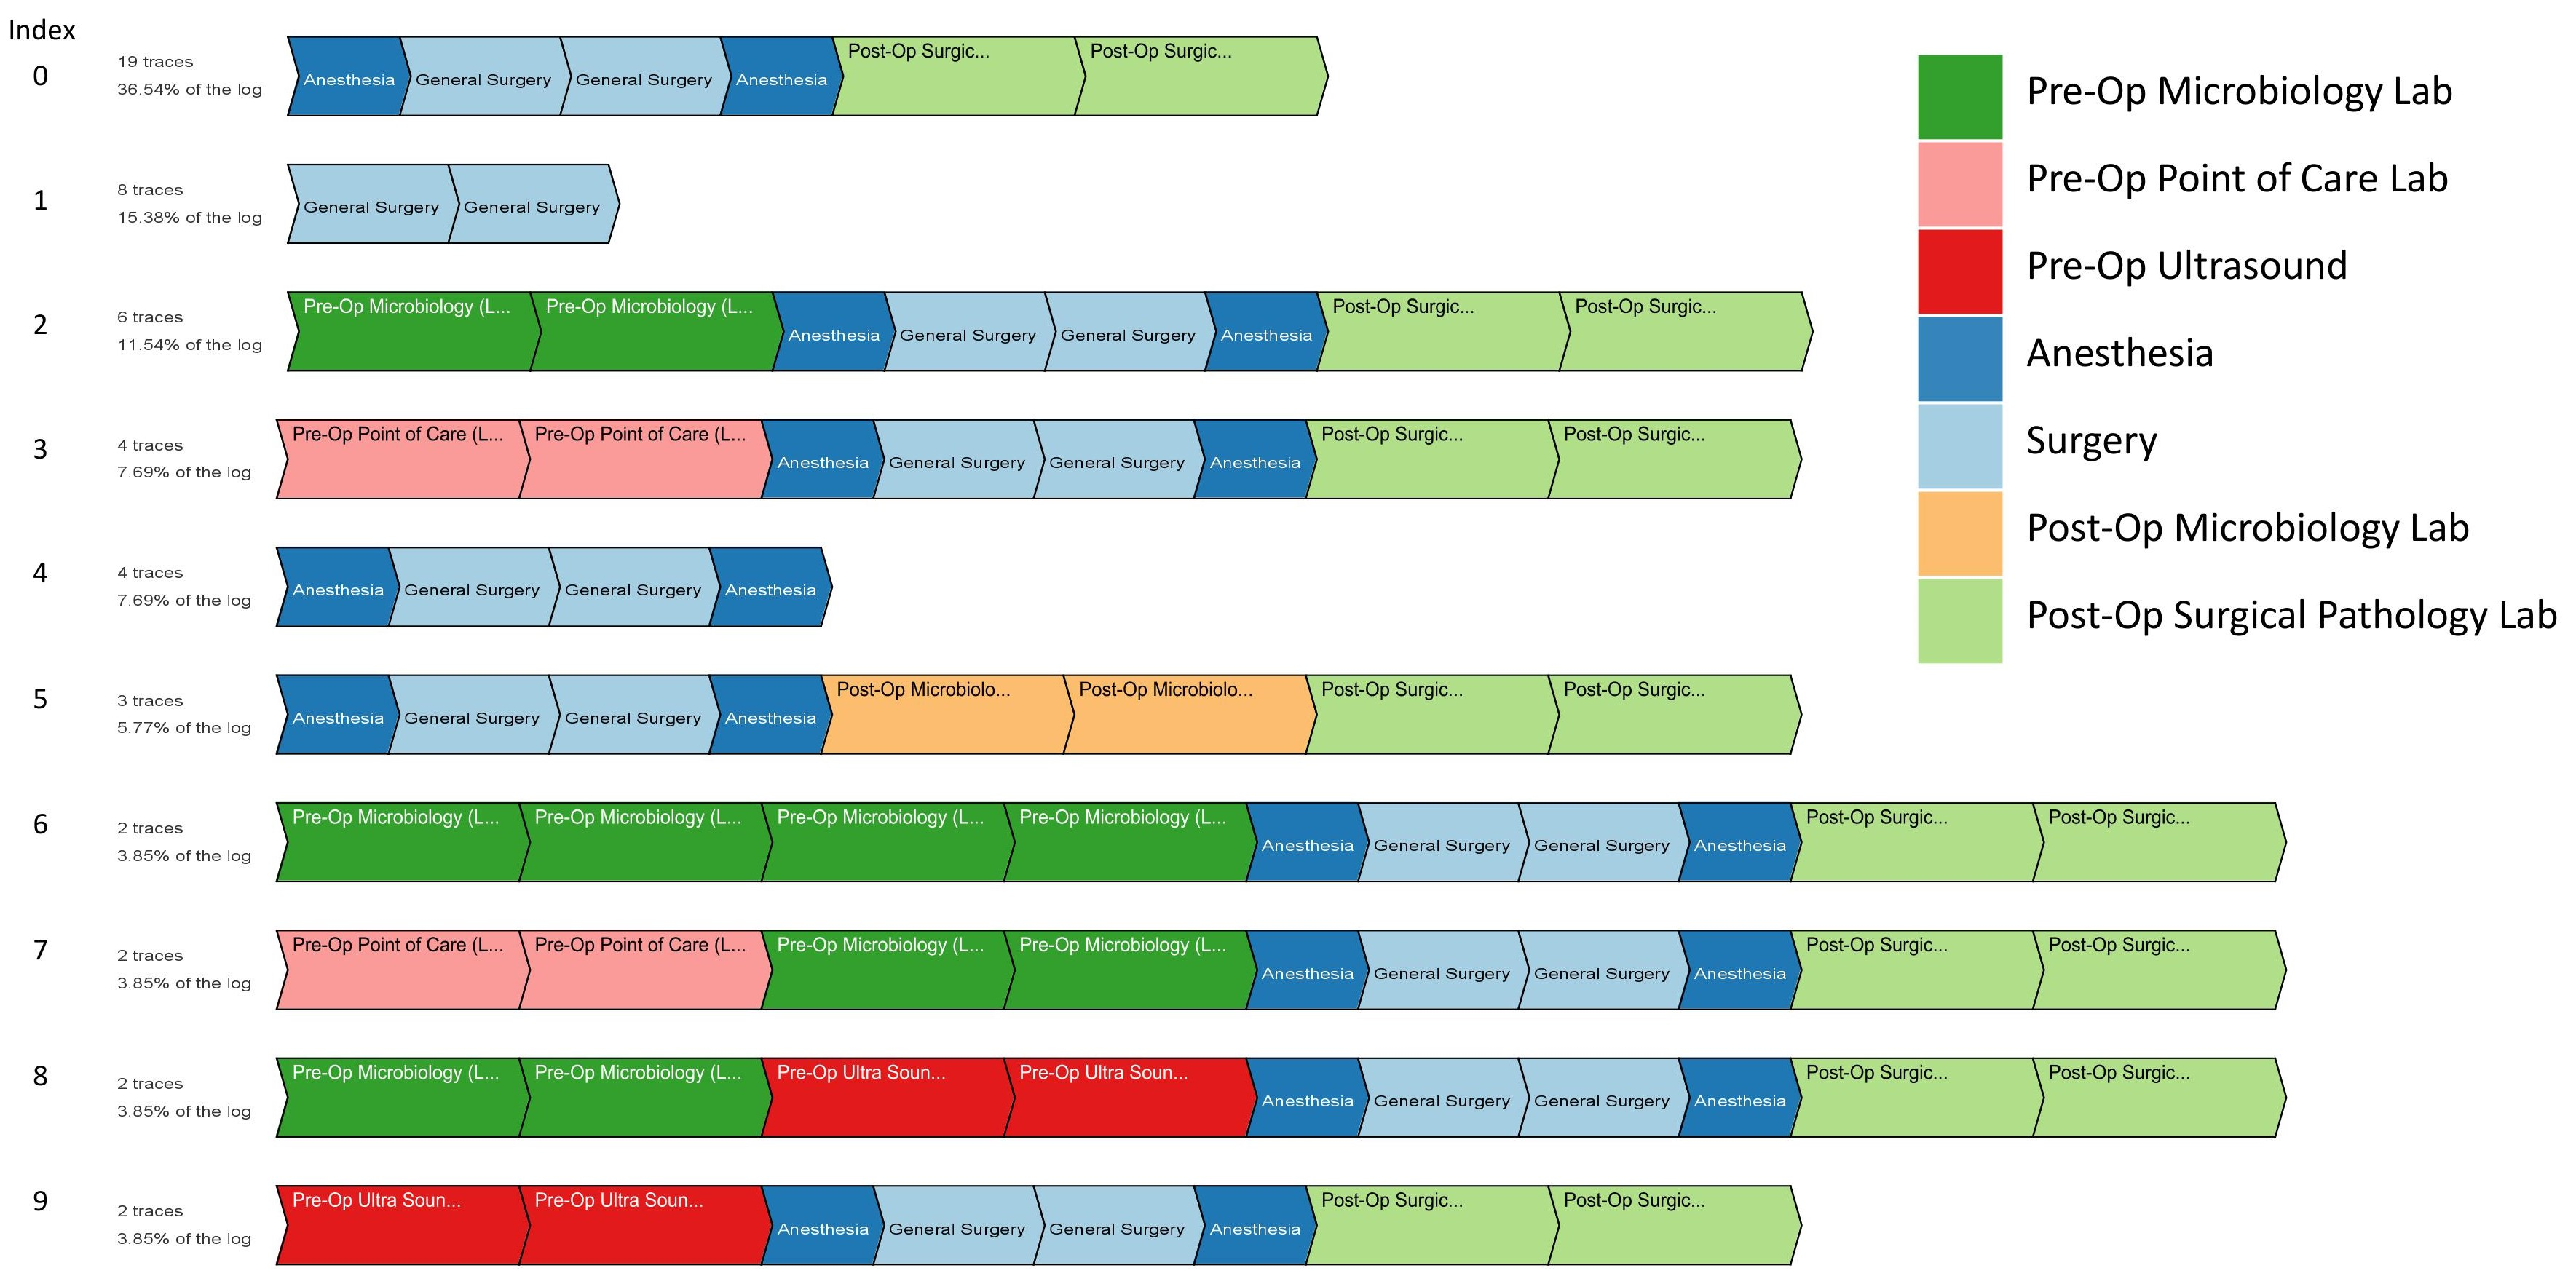
\includegraphics[width=1.5\textwidth]{images/cholecystitis_variant_index_anes.jpg}
\caption{Cholecystitis pathway variants auto-generated by ProM and appended with a legend. The top three pathway variants account for approximately 63\% of the patient traces. The statistics on the left are not readable in this reproduction but are listed in Table \ref{table:cholecystitis variant table}.}
\label{fig:cholecystitis pathway variants}
\end{figure}

\begin{table}[t]
\centering
\caption{Number of patient traces that follow each cholecystitis pathway variant.}
\label{table:cholecystitis variant table}
\begin{tabular}{ l l l }
 \hline
 Index & Number of Patient Traces & Percentage of Patients \% \\ 
 \hline
 0 & 19 & 36.54\\ 
 \hline
 1 & 8 & 15.38\\ 
 \hline
 2 & 6 & 11.54\\ 
 \hline
 3 & 4 & 7.69\\ 
 \hline
 4 & 4 & 7.69\\ 
 \hline
 5 & 3 & 5.77\\ 
 \hline
 6 & 2 & 3.85\\ 
 \hline
 7 & 2 & 3.85\\ 
 \hline
 8 & 2 & 3.85\\ 
 \hline
 9 & 2 & 3.85\\ 
 \hline
\end{tabular}
\end{table}

\subsection{Cholecystitis Pathway Model}
The cholecystitis pathway model visualized by \texttt{`Inductive Visual Miner'} incorporates activities from the `antibiotics' sub-process and the `monitoring labs' sub-process. A breakdown of the reformulated cholecystitis pathway model into one primary pathway and two concurrent sub-processes is shown in Fig.~\ref{fig:cholecystitis pathway model}, and the model notations are summarized in Table \ref{table:notation table}. The first pathway model in Fig.~\ref{fig:cholecystitis pathway model} is the primary pathway, followed by the `antibiotics’ sub-process and the `monitoring labs’ sub-process. Patient traces can execute any combination of the two sub-processes concurrently with the primary pathway. The eight patient traces that follow the second pathway variant (index 1) do not conform to this pathway model because of faulty clinical data. Based on this model, pre-operation haematology and chemistry labs tend to span the entire pre-operation process, while pre-operation antibiotics are taken closer to surgery.

\begin{figure}[t]
\centering
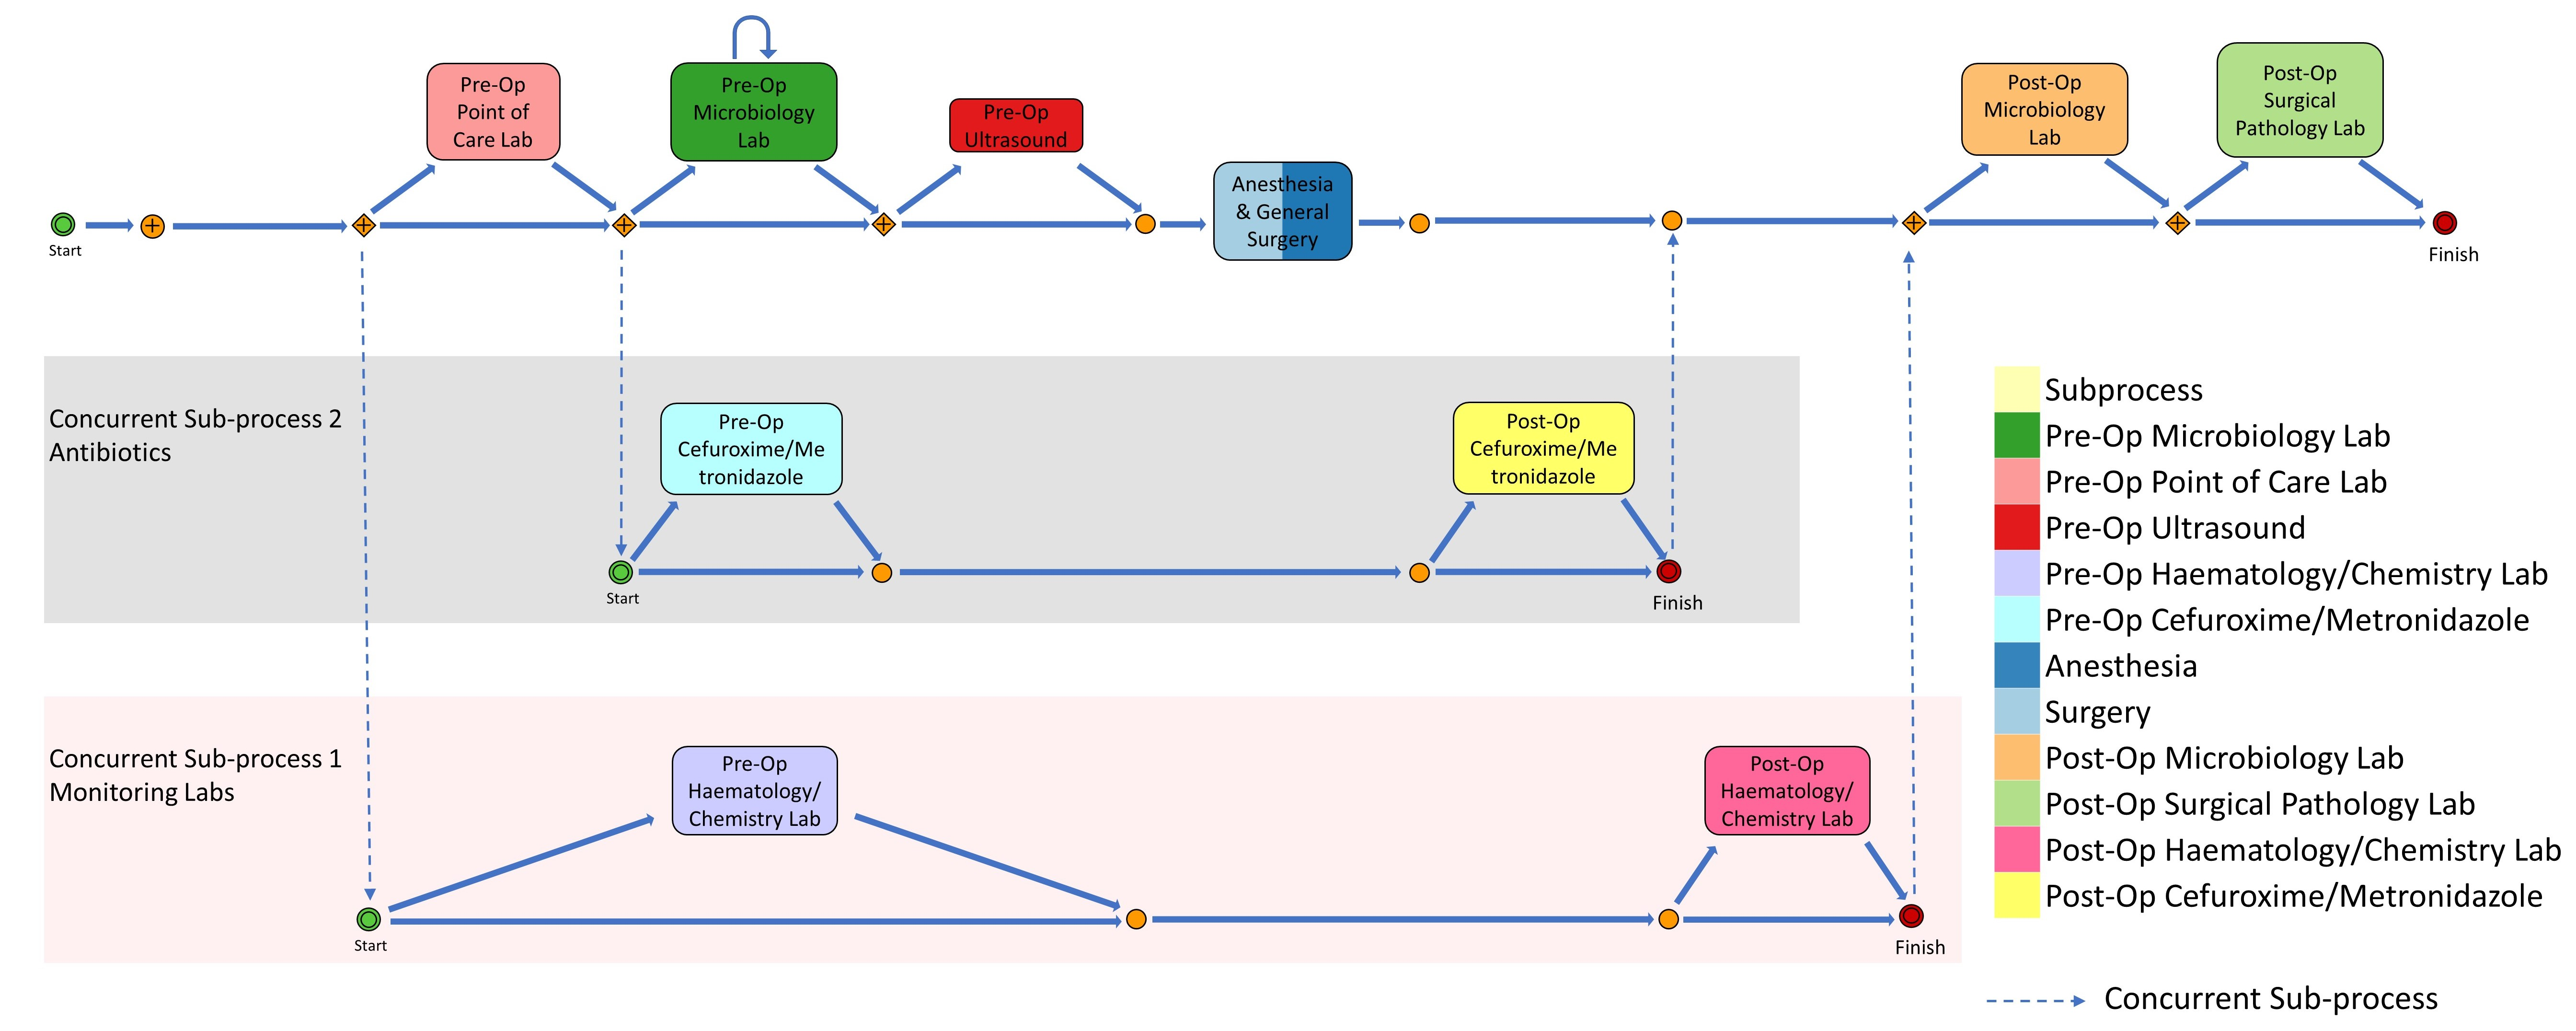
\includegraphics[width=18cm,angle=270]{images/communicative_cholecystitis_process_models_anes.jpg}
\caption{Cholecystitis pathway model. The model is broken down into one primary pathway and two sub-processes.}
\label{fig:cholecystitis pathway model}
\end{figure}